\section{Integration in Other Coordinate Systems}

Choosing coordinates adapted to the region can simplify both the bounds and the integrand. A change of coordinates also changes the area or volume element: substituting for $x$, $y$, and $z$ alone is not enough.

\subsection{Integration in Polar Coordinates}

\begin{definition}{Polar Coordinates and the Area Element}{polar_area_element}
In the plane, write
\[
    x = r\cos\theta,\qquad y = r\sin\theta,\qquad r \geq 0.
\]
Then $x^2 + y^2 = r^2$, and the area element is
\[
    \boxed{\dd{A} = r\,\dd{r}\,\dd{\theta}}.
\]
\end{definition}

A small polar sector has radial width $\Delta r$ and arc length approximately $r\Delta\theta$, so $\Delta A \approx r\Delta r\Delta\theta$. Passing to the Riemann-sum limit gives the factor $r$.

\begin{center}
\begin{tikzpicture}[scale=0.8,>=Stealth]
    % Shade a polar area element
    \filldraw[fill=orange!25,draw=orange!80!black,thick]
    (25:1.5) -- (25:2.5) arc (25:55:2.5) -- (55:1.5) arc (55:25:1.5);
    % Draw axes and radial guides
    \draw[->] (0,0) -- (3,0) node[right] {$x$};
    \draw[->] (0,0) -- (0,2.65) node[above] {$y$};
    \draw[dashed] (0,0) -- (25:2.8);
    \draw[dashed] (0,0) -- (55:2.8);
    \draw[->] (25:0.75) arc (25:55:0.75);
    \node at (40:1.03) {$\Delta\theta$};
    \node[below right] at (25:2) {$\Delta r$};
    \node[above right] at (40:2.5) {$r\Delta\theta$};
    \node at (40:2) {$\Delta A$};
\end{tikzpicture}
\end{center}

\begin{theorem}{Double Integrals in Polar Coordinates}{polar_integration}
Suppose $f$ is continuous on a region $\mathcal{D}$ described by
\[
    \alpha \leq \theta \leq \beta,\qquad
    r_1(\theta) \leq r \leq r_2(\theta),
\]
with nonnegative radial bounds and no overlapping coverage in the interior. Then
\[
    \diint{f(x,y)}
    = \int_\alpha^\beta\int_{r_1(\theta)}^{r_2(\theta)}
    f(r\cos\theta,r\sin\theta)\,r\,\dd{r}\,\dd{\theta}.
\]
\end{theorem}

\clearpage
\begin{example}[A Right Half-Annulus]
Let $\mathcal{R}$ be the region between $x^2 + y^2 = 1$ and $x^2 + y^2 = 4$ with $x > 0$. Set up an integral for $\displaystyle\xiint{\mathcal{R}}{x}$.
\end{example}

\begin{sol}
The circles become $r = 1$ and $r = 2$. Since $x = r\cos\theta > 0$, we may use
\[
    1 \leq r \leq 2,\qquad -\frac{\pi}{2} \leq \theta \leq \frac{\pi}{2}.
\]
Including the boundary $x = 0$ does not affect the integral. Thus
\begin{align*}
    \xiint{\mathcal{R}}{x}
    &= \int_{-\pi/2}^{\pi/2}\int_1^2
    (r\cos\theta)r\,\dd{r}\,\dd{\theta}\\
    &= \left(\int_1^2r^2\,\dd{r}\right)
    \left(\int_{-\pi/2}^{\pi/2}\cos\theta\,\dd{\theta}\right)
    = \frac{7}{3}\cdot 2 = \frac{14}{3}.
\end{align*}
\end{sol}

\begin{example}[Population in a Half-Annulus]
A city occupies the same region $\mathcal{R}$, with distances in kilometers. Its population density is $|xy|$ thousand people per square kilometer. Write an iterated integral for the population.
\end{example}

\begin{sol}
The density becomes
\[
    |xy| = |r^2\cos\theta\sin\theta|.
\]
Consequently, the population in thousands of people is
\begin{align*}
    P &= \int_{-\pi/2}^{\pi/2}\int_1^2
    r^3|\cos\theta\sin\theta|\,\dd{r}\,\dd{\theta}\\
    &= 2\int_0^{\pi/2}\int_1^2
    r^3\cos\theta\sin\theta\,\dd{r}\,\dd{\theta}\\
    &= 2\cdot\frac{15}{4}\cdot\frac{1}{2} = \frac{15}{4}.
\end{align*}
The population is therefore $3750$ people. The extra factor $r$ comes from $\dd{A}$, in addition to the $r^2$ in the density.
\end{sol}

\clearpage
\subsection{Integration in Cylindrical Coordinates}

\begin{definition}{Cylindrical Coordinates and the Volume Element}{cylindrical_volume_element}
Cylindrical coordinates combine polar coordinates in the $xy$-plane with height $z$:
\[
    x = r\cos\theta,\qquad y = r\sin\theta,\qquad z = z.
\]
Here $r \geq 0$ is the distance from the $z$-axis, and
\[
    \boxed{\dd{V} = r\,\dd{r}\,\dd{\theta}\,\dd{z}}.
\]
\end{definition}

A small cylindrical wedge has dimensions approximately $\Delta r$, $r\Delta\theta$, and $\Delta z$. Hence
\[
    \Delta V \approx (\Delta r)(r\Delta\theta)(\Delta z).
\]
Equivalently, $\dd{V} = \dd{A}\,\dd{z}$ with the polar area element $\dd{A} = r\,\dd{r}\,\dd{\theta}$.

\begin{theorem}{Triple Integrals in Cylindrical Coordinates}{cylindrical_integration}
If a solid $\mathcal{W}$ is described by
\[
    \alpha \leq \theta \leq \beta,\qquad
    r_1(\theta) \leq r \leq r_2(\theta),\qquad
    z_1(r,\theta) \leq z \leq z_2(r,\theta),
\]
then, for continuous $f$,
\[
    \wiiint{f(x,y,z)}
    = \int_\alpha^\beta\int_{r_1(\theta)}^{r_2(\theta)}
    \int_{z_1(r,\theta)}^{z_2(r,\theta)}
    f(r\cos\theta,r\sin\theta,z)\,r\,\dd{z}\,\dd{r}\,\dd{\theta}.
\]
The order may be changed when the bounds are rewritten accordingly.
\end{theorem}

Cylindrical coordinates are useful when boundaries involve $x^2 + y^2$: for instance, $x^2 + y^2 = a^2$ becomes $r = a$, and $z = x^2 + y^2$ becomes $z = r^2$.

\textbf{Choosing the axis.} For a cylinder about the $x$-axis, use polar coordinates in the $yz$-plane:
\[
    y = r\cos\theta,\qquad z = r\sin\theta,\qquad
    \dd{V} = r\,\dd{r}\,\dd{\theta}\,\dd{x}.
\]

\clearpage
\begin{example}[Particles Inside a Cylindrical Tube]
A tube is bounded by $y^2 + z^2 = 4$, $x = 0$, and $x = 2$, with distances in centimeters. The stated particle density is $f(x,y,z) = 1 + x^2 + yz$ particles per cubic centimeter. Evaluate the integral of $f$ over the tube.
\end{example}

\begin{sol}
The tube's axis is the $x$-axis. Use
\[
    y = r\cos\theta,\qquad z = r\sin\theta,
\]
so that the solid is described by
\[
    0 \leq x \leq 2,\qquad 0 \leq r \leq 2,\qquad
    0 \leq \theta \leq 2\pi.
\]
Then
\begin{align*}
    N &= \int_0^2\int_0^{2\pi}\int_0^2
    \bigl(1 + x^2 + r^2\cos\theta\sin\theta\bigr)
    r\,\dd{r}\,\dd{\theta}\,\dd{x}\\
    &= \int_0^2\int_0^{2\pi}
    \bigl(2(1 + x^2) + 4\cos\theta\sin\theta\bigr)
    \,\dd{\theta}\,\dd{x}\\
    &= 4\pi\int_0^2(1 + x^2)\,\dd{x}
    = 4\pi\left[x + \frac{x^3}{3}\right]_0^2
    = \boxed{\frac{56\pi}{3}}.
\end{align*}
The $yz$ term integrates to zero because
\[
    \int_0^{2\pi}\cos\theta\sin\theta\,\dd{\theta} = 0.
\]
This also follows from symmetry: reflecting $y$ to $-y$ preserves the tube and reverses the sign of $yz$.
\end{sol}

\textbf{Modeling note.} The lecture's stated density can be negative inside the tube; for instance, $f(0,1,-\sqrt{2}) = 1 - \sqrt{2} < 0$. Thus $56\pi/3$ is the value of the stated integral, but a physical particle-density model would require a nonnegative function.

\clearpage
\subsection{Integration in Spherical Coordinates}

\begin{definition}{Spherical Coordinates and the Volume Element}{spherical_volume_element}
Using $\rho$ for distance from the origin, $\theta$ for the angle in the $xy$-plane, and $\phi$ for the angle measured down from the positive $z$-axis,
\[
    x = \rho\sin\phi\cos\theta,\qquad
    y = \rho\sin\phi\sin\theta,\qquad
    z = \rho\cos\phi.
\]
Here $\rho \geq 0$, $0 \leq \theta < 2\pi$, $0 \leq \phi \leq \pi$, and
\[
    x^2 + y^2 + z^2 = \rho^2,\qquad r = \rho\sin\phi,
\]
The volume element is
\[
    \boxed{\dd{V} = \rho^2\sin\phi\,\dd{\rho}\,\dd{\phi}\,\dd{\theta}}.
\]
\end{definition}

\noindent
\begin{minipage}[c]{0.53\textwidth}
The three local side lengths multiply to give the volume element. The circle traced by changing $\theta$ has radius $\rho\sin\phi$, which explains the factor $\sin\phi$.
\end{minipage}\hfill
\begin{minipage}[c]{0.44\textwidth}
\centering
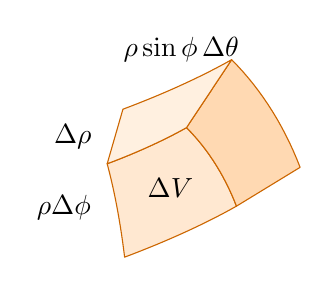
\begin{tikzpicture}[
    scale=1.1,
    line cap=round,
    line join=round,
    declare function={
        sx(\r,\t,\p) = \r*sin(\p)*(-0.6*cos(\t) + sin(\t));
        sy(\r,\t,\p) = \r*(cos(\p) + sin(\p)*(-0.45*cos(\t) + 0.15*sin(\t)));
    }
]
    % Draw three curved faces of a small spherical wedge.
    \filldraw[fill=orange!18,draw=orange!80!black]
        plot[domain=45:75,samples=16] ({sx(2.7,\x,40)},{sy(2.7,\x,40)})
        -- plot[domain=40:65,samples=16] ({sx(2.7,75,\x)},{sy(2.7,75,\x)})
        -- plot[domain=75:45,samples=16] ({sx(2.7,\x,65)},{sy(2.7,\x,65)})
        -- plot[domain=65:40,samples=16] ({sx(2.7,45,\x)},{sy(2.7,45,\x)}) -- cycle;
    \filldraw[fill=orange!30,draw=orange!80!black]
        ({sx(2.7,75,40)},{sy(2.7,75,40)})
        -- ({sx(3.7,75,40)},{sy(3.7,75,40)})
        -- plot[domain=40:65,samples=16] ({sx(3.7,75,\x)},{sy(3.7,75,\x)})
        -- ({sx(2.7,75,65)},{sy(2.7,75,65)})
        -- plot[domain=65:40,samples=16] ({sx(2.7,75,\x)},{sy(2.7,75,\x)}) -- cycle;
    \filldraw[fill=orange!12,draw=orange!80!black]
        ({sx(2.7,45,40)},{sy(2.7,45,40)})
        -- ({sx(3.7,45,40)},{sy(3.7,45,40)})
        -- plot[domain=45:75,samples=16] ({sx(3.7,\x,40)},{sy(3.7,\x,40)})
        -- ({sx(2.7,75,40)},{sy(2.7,75,40)})
        -- plot[domain=75:45,samples=16] ({sx(2.7,\x,40)},{sy(2.7,\x,40)}) -- cycle;
    % Label only the three local side lengths and the volume element.
    \path ({sx(2.7,45,40)},{sy(2.7,45,40)})
        -- ({sx(3.7,45,40)},{sy(3.7,45,40)}) node[midway,left=5pt] {$\Delta\rho$};
    \node[left=6pt] at ({sx(2.7,45,52.5)},{sy(2.7,45,52.5)}) {$\rho\Delta\phi$};
    \node[above=5pt] at ({sx(3.7,60,40)},{sy(3.7,60,40)}) {$\rho\sin\phi\,\Delta\theta$};
    \node at ({sx(2.7,60,53)},{sy(2.7,60,53)}) {$\Delta V$};
\end{tikzpicture}

\end{minipage}

\begin{theorem}{Triple Integrals in Spherical Coordinates}{spherical_integration}
Let $\mathcal{W}$ be described by
\[
    \alpha \leq \theta \leq \beta,\qquad
    \phi_1(\theta) \leq \phi \leq \phi_2(\theta),\qquad
    \rho_1(\phi,\theta) \leq \rho \leq \rho_2(\phi,\theta).
\]
For continuous $f$,
\begin{align*}
    \wiiint{f(x,y,z)}
    &= \int_\alpha^\beta\int_{\phi_1(\theta)}^{\phi_2(\theta)}
    \int_{\rho_1(\phi,\theta)}^{\rho_2(\phi,\theta)}\\
    &\quad f(\rho\sin\phi\cos\theta,\rho\sin\phi\sin\theta,\rho\cos\phi)
    \,\rho^2\sin\phi\,\dd{\rho}\,\dd{\phi}\,\dd{\theta}.
\end{align*}
\end{theorem}



\clearpage
\begin{example}[Volume of the Unit Ball]
Let $\mathcal{B}$ be the ball of radius $1$ centered at the origin. Find its volume.
\end{example}

\begin{sol}
The ball is $0 \leq \rho \leq 1$, $0 \leq \phi \leq \pi$, $0 \leq \theta \leq 2\pi$. Therefore,
\begin{align*}
    \operatorname{Vol}(\mathcal{B})
    &= \int_0^{2\pi}\int_0^\pi\int_0^1
    \rho^2\sin\phi\,\dd{\rho}\,\dd{\phi}\,\dd{\theta}\\
    &= 2\pi\left[-\cos\phi\right]_0^\pi
    \left[\frac{\rho^3}{3}\right]_0^1
    = \boxed{\frac{4\pi}{3}}.
\end{align*}
\end{sol}

\begin{example}[Average Height of a Truncated Cone]
Let $\mathcal{U}$ be the solid inside $z^2 = x^2 + y^2$ between $z = 1$ and $z = 2$. Find the average $z$-coordinate of points in $\mathcal{U}$.
\end{example}

\begin{sol}
Since $z > 0$, the solid lies inside the upper cone. In spherical coordinates,
\[
    0 \leq \theta \leq 2\pi,\qquad
    0 \leq \phi \leq \frac{\pi}{4},\qquad
    \sec\phi \leq \rho \leq 2\sec\phi.
\]
The radial bounds come from $1 \leq \rho\cos\phi \leq 2$. Thus
\begin{align*}
    V &= \int_0^{2\pi}\int_0^{\pi/4}\int_{\sec\phi}^{2\sec\phi}
    \rho^2\sin\phi\,\dd{\rho}\,\dd{\phi}\,\dd{\theta}\\
    &= \frac{14\pi}{3}\int_0^{\pi/4}\frac{\sin\phi}{\cos^3\phi}\,\dd{\phi}
    = \frac{14\pi}{3}\left[\frac{1}{2\cos^2\phi}\right]_0^{\pi/4}
    = \frac{7\pi}{3},\\
    \xiiint{\mathcal{U}}{z}
    &= \int_0^{2\pi}\int_0^{\pi/4}\int_{\sec\phi}^{2\sec\phi}
    (\rho\cos\phi)\rho^2\sin\phi\,\dd{\rho}\,\dd{\phi}\,\dd{\theta}\\
    &= \frac{15\pi}{2}\int_0^{\pi/4}\frac{\sin\phi}{\cos^3\phi}\,\dd{\phi}
    = \frac{15\pi}{4}.
\end{align*}
Hence
\[
    z_{\mathrm{avg}} = \frac{1}{V}\xiiint{\mathcal{U}}{z}
    = \frac{15\pi/4}{7\pi/3} = \boxed{\frac{45}{28}}.
\]
\end{sol}

\clearpage
\subsection{Choosing a Coordinate System}

The same solid can admit several useful descriptions. For the truncated cone above, cylindrical coordinates give the simpler bounds
\[
    1 \leq z \leq 2,\qquad 0 \leq r \leq z,\qquad
    0 \leq \theta \leq 2\pi.
\]
As a check,
\[
    V = \int_1^2\int_0^{2\pi}\int_0^z r\,\dd{r}\,\dd{\theta}\,\dd{z}
    = \pi\int_1^2 z^2\,\dd{z} = \frac{7\pi}{3},
\]
\[
    \xiiint{\mathcal{U}}{z}
    = \int_1^2\int_0^{2\pi}\int_0^z zr\,\dd{r}\,\dd{\theta}\,\dd{z}
    = \pi\int_1^2 z^3\,\dd{z} = \frac{15\pi}{4}.
\]
Both methods yield $z_{\mathrm{avg}} = 45/28$.

\begin{center}
\renewcommand{\arraystretch}{1.35}
\begin{tabular}{lll}
\hline
\textbf{Coordinates} & \textbf{Typical geometry} & \textbf{Area/volume factor}\\
\hline
Polar & Disks, annuli, sectors & $r$\\
Cylindrical & Cylinders, axial symmetry & $r$\\
Spherical & Balls, spherical shells, cones & $\rho^2\sin\phi$\\
\hline
\end{tabular}
\end{center}

\textbf{Setting up an integral.}
\begin{enumerate}
    \item Sketch the region and identify its axis or symmetry.
    \item Rewrite all boundary equations in the chosen coordinates.
    \item Choose an integration order and determine bounds from outside inward.
    \item Replace every occurrence of the original coordinates in the integrand.
    \item Include the area or volume factor exactly once, then evaluate from inside outward.
\end{enumerate}

\textbf{Common pitfalls.} In spherical coordinates, $\rho$ is distance from the origin, whereas $r = \rho\sin\phi$ is distance from the $z$-axis. The angle $\phi$ is measured from the positive $z$-axis, so the upper half-space has $0 \leq \phi \leq \pi/2$. Bounds must cover the region once; splitting a region into pieces may be necessary.
